\subsection{DFS-based approach}
	\begin{frame}
		\begin{itemize}
			\item We can exploit the information provided by $\overline G$ and avoid generating orders which are guaranteed sub-optimal
			\item Assume \alert{best parent set} is unique
			\item Consider two variables $X_i$ and $X_j$ in $\overline G$, where $X_j$ is parent of $X_i$, but there is no arc from $X_i$ to $X_j$
			\item No optimal ordering can have $X_i$ preceding $X_j$
		\end{itemize}
		The number of these orderings can be much smaller than the full space of orderings
	\end{frame}
	\begin{frame}{Example}
		\begin{columns}
			\begin{column}{.48\textwidth}
				\begin{figure}
					\centering
					\begin{tikzpicture}[ scale = 0.6 ]
	\tikzset{ vertex/.style = { shape = circle , draw , minimum size = 1.5em } }
	\tikzset{ edge/.style = { ->,> = latex' } }
	% vertices
	\node[ vertex ] (A) at  ( 3 , 4 ) { ${A}$ } ;
	\node[ vertex ] (B) at  ( 0 , 0 ) { ${B}$ } ;
	\node[ vertex ] (C) at  ( 3 , 0 ) { ${C}$ } ;
	\node[ vertex ] (D) at  ( 6 , 0 ) { ${D}$ } ;

	%edges
	\draw[ edge ] (A) to (B) ;
%	\draw[ edge ] (B) to[in=180,out=90] (A) ;
	\draw[ edge ] (A) to (C) ;
	\draw[ edge ] (A) to (D) ;
%	\draw[ edge ] (D) to[in=0,out=90] (A) ;
	\draw[ edge ] (C) to (D) ; 
	\draw[ edge ] (B) to[in=-135,out=-45] (D) ;
\end{tikzpicture}
				\end{figure}
				\centering
				Graph $\overline G$
			\end{column}
			\begin{column}{.48\textwidth}
				\begin{figure}
					\centering
					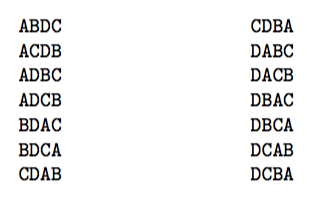
\includegraphics{images/dfsorders}
				\end{figure}
				\centering
				Possible orders from $\overline G$
			\end{column}
		\end{columns}
	\end{frame}
	\begin{frame}
		\begin{block}{The algorithm}
			\begin{itemize}
				\item Take as input $\overline G$ and mark all nodes unvisited
				\item Start with an empty list $L$
				\item While there is an unvisited node
				\begin{itemize}
					\item Select an unvisited $X_i$ uniformly random
					\item Perform a depth-first search (DFS) rooted at $X_i$ and add to $L$ the visited nodes
				\end{itemize}
				\item Return $L$
			\end{itemize}
		\end{block}
	\end{frame}